\begin {itemize}
\item Use Cases
\begin {itemize}
\item {createBuzzSpace}\\
This is the service which enables a lecturer to create a Buzz space for a particular module they present.
\begin {itemize}
\item Pre-conditions:\\
-buzzSpaceExists (should not be able to create a duplicate buzz space) (implemented, was unable to create a space that already existed)\\
-moduleNotActive (for the current year) (not implemented, was able to create a space for a non existent module)\\
-notAuthorized (only an authorized user can create a buzz space) (not implemented, was able to create a space without signing in as a lecturer)\\

\item Post-conditions:\\
-storeBuzzSpace (persist the new buzz space)(implemented, new buzz space was reflected in system once user is returned to home page)\\
-lecturer registered on the buzz space (not implemented)\\
-lecturer assigned as administrator of the buzz space (not implemented)\\
-Create welcome message as root thread for the buzz space (not implemented)\\
\end {itemize}

\begin{figure}[h!]
  \centering
    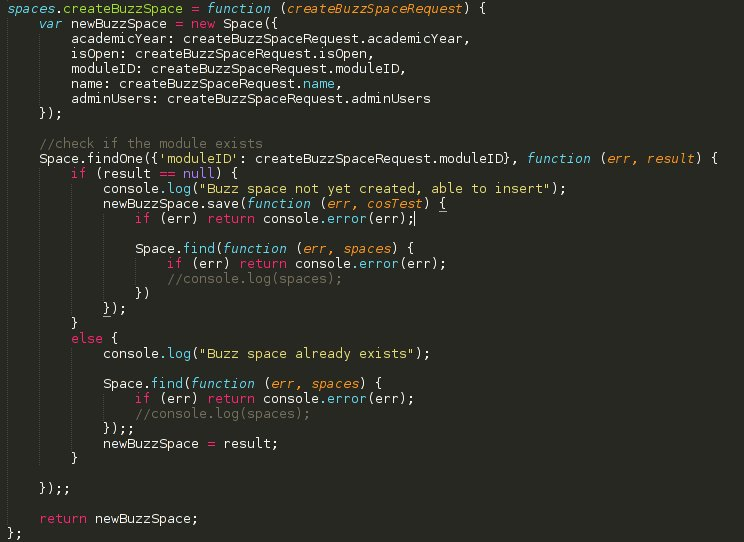
\includegraphics[width=0.85\textwidth]{buzzSpaceCreationCode} 
\end{figure}

\begin{figure}[h!]
  \centering
    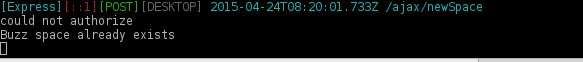
\includegraphics[width=0.85\textwidth]{buzzSpaceCreationFailToCreateDuplicate} 
\end{figure}

\begin{figure}[h!]
  \centering
    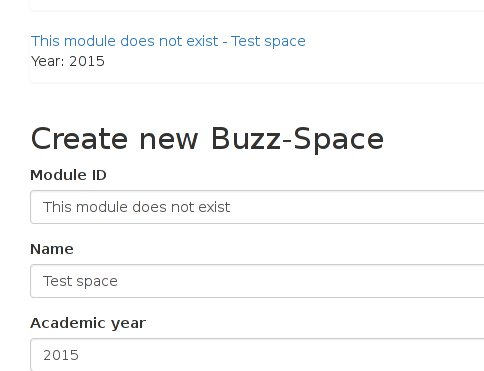
\includegraphics[width=0.85\textwidth]{buzzSpaceCreationModuleNotActive} 
\end{figure}

\begin{figure}[h!]
  \centering
    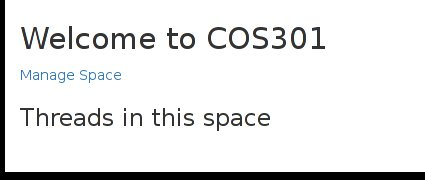
\includegraphics[width=0.85\textwidth]{buzzSpaceCreationNoRootThread} 
\end{figure}


\item {closeBuzzSpace}\\
This is the service used to set a buzz space to inactive.
\begin {itemize}
\item Pre-conditions: \\
-noSuchBuzzSpace (if buzz space to be closed does not exist then one can't close it) (was unable to find a non existent buzz space to test this)\\
        -notAuthorized (only an admin user of a buzz space can close the buzz space) (not implemented, was able to close a space I was not an admin for)\\
\item Post-conditions:\\
-buzz space no longer active (reflected upon returning to the home page)\\
\end{itemize}

\begin{figure}[h!]
  \centering
    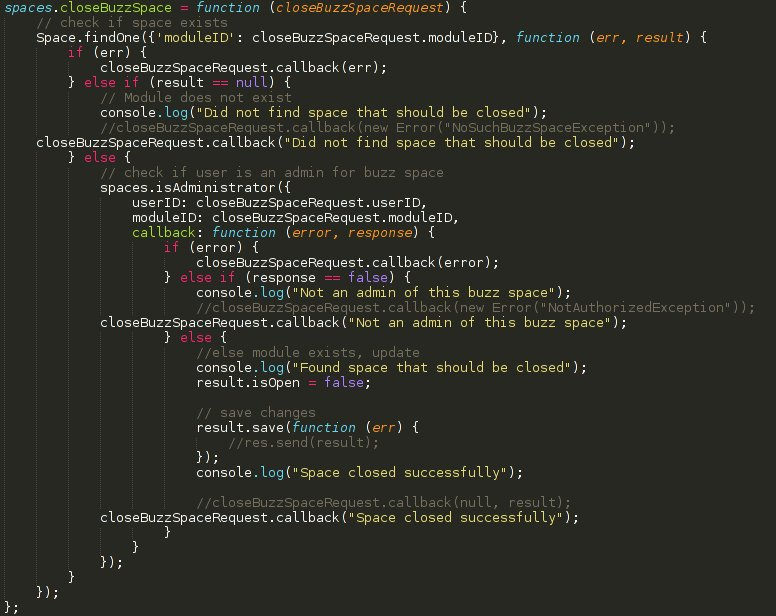
\includegraphics[width=0.85\textwidth]{buzzSpaceCloseCode} 
\end{figure}

\begin{figure}[h!]
  \centering
    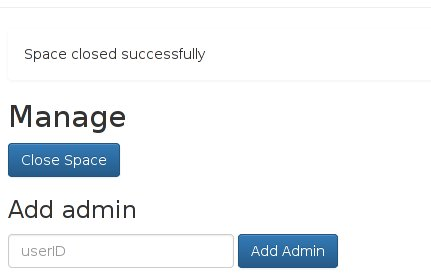
\includegraphics[width=0.85\textwidth]{buzzSpaceCloseSuccessful} 
\end{figure}

\begin{figure}[h!]
  \centering
    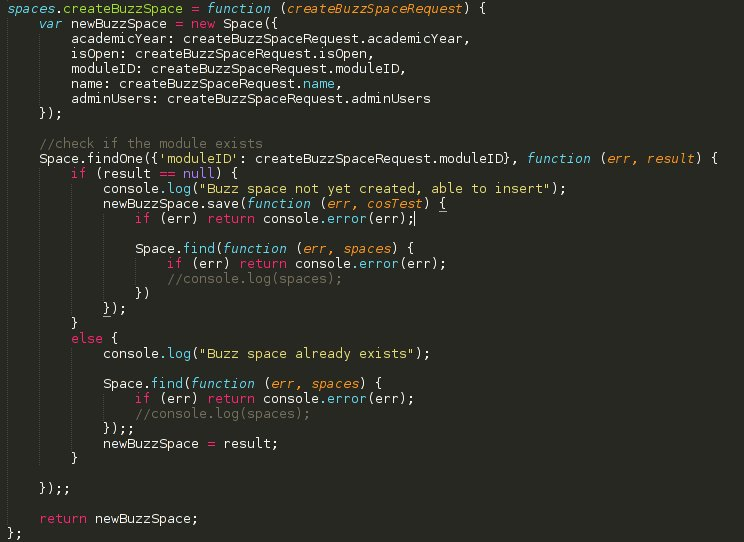
\includegraphics[width=0.85\textwidth]{buzzSpaceCreationCode} 
\end{figure}

\begin{figure}[h!]
  \centering
    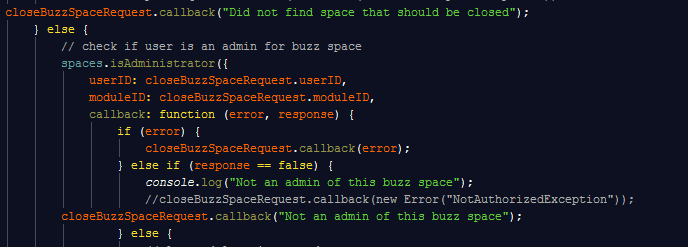
\includegraphics[width=0.85\textwidth]{closeBuzzSpace} 
\end{figure}

\item {registerOnBuzzSpace}\\
This service is used to create a profile for a user on a particular buzz space.
\begin {itemize}
\item Pre-conditions: \\
-notAuthorized (user is registered for the module to which the space is associated) (not implemented, was able to register a fake user successfully)\\
        -buzz space active (implemented, only able to access register for spaces which are active on home page)\\
\item Post-conditions: \\
 -user profile persisted to database (implemented) (screenshots provided for proof)\\
\end{itemize}

\begin{figure}[h!]
  \centering
    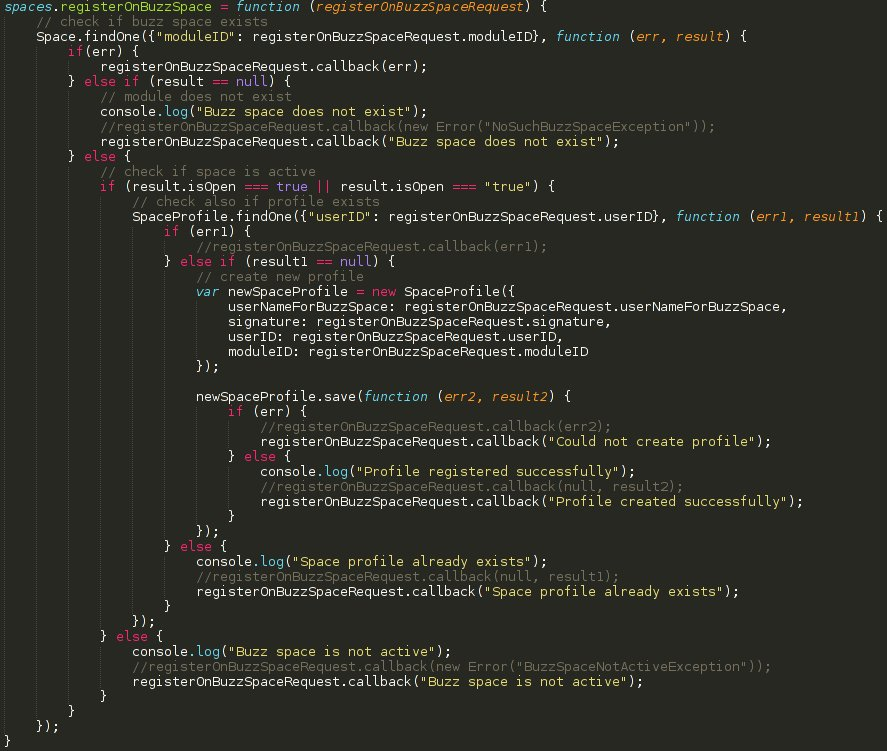
\includegraphics[width=0.85\textwidth]{buzzSpaceRegisterCode} 
\end{figure}

\begin{figure}[h!]
  \centering
    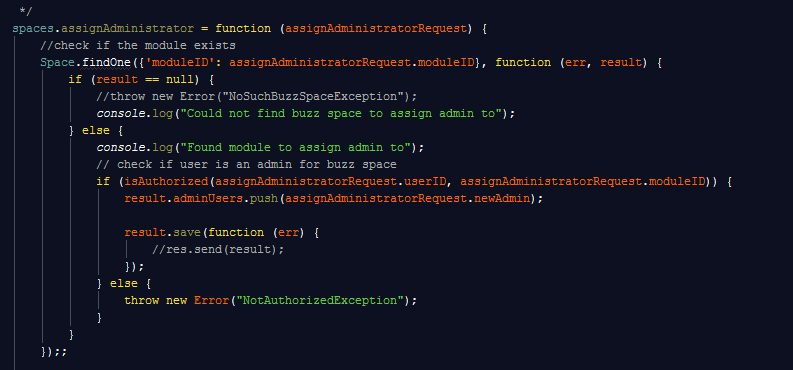
\includegraphics[width=0.85\textwidth]{addAdmin} 
\end{figure}

\item{getProfileForUser}
Simply returns the profile the user has on the buzz space\\
Code found but no functional implementation exists in the system that could be tested \\
\end{itemize}
\end{itemize}
